\documentclass[aspectratio=169, table]{beamer}

\usepackage{colortbl}
\usepackage{xcolor}
\usepackage{listings}
\usepackage{pgfplots}
\usepgfplotslibrary{polar}
\usepackage{tikz}
\usetikzlibrary{shapes.geometric,
	positioning, shapes, shapes.multipart, backgrounds, arrows.meta, calc, fit, trees}

\makeatletter
\def\input@path{{../theme/}}
\makeatother
\graphicspath{{../theme/}}
\usetheme{Pradita}

\lstdefinelanguage{xml}{
	keywords={},
	basicstyle=\ttfamily\scriptsize,
	keywordstyle=\color{blue}\bfseries,
	sensitive=true,
	commentstyle=\color{gray}\ttfamily,
	stringstyle=\color{purple}\ttfamily,
	numbers=left,
	numberstyle=\tiny\color{gray},
	breaklines=true,
	frame=lines,
	backgroundcolor=\color{lightgray!10},
	tabsize=2,
	morecomment=[s]{<!--}{-->},
	morestring=[b]",
	morestring=[b]',
	showstringspaces=false
}

\lstdefinelanguage{java}{
  keywords={package,import,public,class,interface,extends,implements,
            return,new,null,true,false,void,if,else,for,while,static,
            final,private,protected,override,Override,String,throws,Exception},
  keywordstyle=\color{blue}\bfseries,
  sensitive=true,
  comment=[l]{//},
  morecomment=[s]{/*}{*/},
  commentstyle=\color{gray}\ttfamily\itshape,
  stringstyle=\color{purple}\ttfamily,
  morestring=[b]",
  basicstyle=\ttfamily\scriptsize,
  numbers=left,
  numberstyle=\tiny\color{gray},
  breaklines=true,
  frame=lines,
  backgroundcolor=\color{lightgray!10},
  showstringspaces=false
}

\lstdefinelanguage{atl}{
  keywords={module,create,from,rule,to,helper,context,def,do,Sequence,Collection,Boolean},
  keywordstyle=\color{blue}\bfseries,
  sensitive=true,
  comment=[l]{--},
  commentstyle=\color{gray}\ttfamily\itshape,
  stringstyle=\color{purple}\ttfamily,
  morestring=[b]',
  basicstyle=\ttfamily\scriptsize,
  numbers=left,
  numberstyle=\tiny\color{gray},
  breaklines=true,
  frame=lines,
  backgroundcolor=\color{lightgray!10},
  showstringspaces=false
}

\lstdefinelanguage{etl}{
  keywords={rule,transform,to,guard,operation,return,post,var,new,for,in,not,and},
  keywordstyle=\color{blue}\bfseries,
  sensitive=true,
  comment=[l]{//},
  morecomment=[s]{/*}{*/},
  commentstyle=\color{gray}\ttfamily\itshape,
  stringstyle=\color{purple}\ttfamily,
  morestring=[b]",
  basicstyle=\ttfamily\scriptsize,
  numbers=left,
  numberstyle=\tiny\color{gray},
  breaklines=true,
  frame=lines,
  backgroundcolor=\color{lightgray!10},
  showstringspaces=false
}

\subtitle{IT30213 - Advanced Software Engineering \& DevOps}
\title{\Huge Model-to-Model\vspace{8pt}\\
	Transformation}
\author{\textbf{Alfa Yohannis}}

\begin{document}

\frame{\titlepage}

\begin{frame}[fragile]
	\frametitle{Contents}
	\vspace{20pt}
	\begin{columns}[t]
		\column{0.5\textwidth}
		\tableofcontents[sections={1-5}]

		\column{0.5\textwidth}
		\tableofcontents[sections={6-11}]
	\end{columns}
\end{frame}

\begin{frame}{\hfill}
	\centering
	\Huge{\textbf{Bagaimana jika suatu model perlu ditransformasi ke model lain untuk keperluan tertentu (misalnya karena kebutuhan standard)?}}
\end{frame}

% ============================================================
\section{Tujuan Pembelajaran}
\begin{frame}{\hfill}
	\centering
	\Huge{\textbf{Tujuan Pembelajaran}}
\end{frame}

\begin{frame}{Tujuan Pembelajaran}
\vspace{6pt}
Setelah sesi ini, mahasiswa diharapkan mampu:
\begin{enumerate}
  \item Menjelaskan konsep transformasi model-ke-model (M2M) dalam konteks \textit{Model-Driven Engineering}, termasuk peran metamodel sumber dan target.
  \item Menerapkan transformasi model menggunakan ATL (deklaratif) dan ETL (hibrid imperatif-deklaratif) untuk mengonversi model MediaFlow menjadi UML Activity Diagram.
  \item Menganalisis \textit{trade-off} antara pendekatan deklaratif dan imperatif dalam penulisan aturan transformasi.
\end{enumerate}
\end{frame}

% ============================================================
\section{Pendahuluan}
\begin{frame}{\hfill}
	\centering
	\Huge{\textbf{Pendahuluan}}
\end{frame}

\begin{frame}{Posisi M2M dalam Siklus MDE}
\vspace{6pt}
\begin{columns}[T]
\column{0.5\textwidth}
\textbf{Bab Sebelumnya}
\begin{itemize}
  \item Bab 8: Metamodel (\texttt{mediaflow.ecore})
  \item Bab 9: Textual DSL (ANTLR, Xtext, Langium)
  \item Bab 10: Visual DSL (Eclipse Sirius)
\end{itemize}

\vspace{6pt}
\textbf{Fokus:} \textit{authoring} model --- bagaimana model dibuat, diedit, dan disimpan.

\column{0.5\textwidth}
\textbf{Bab Ini: M2M Transformation}
\begin{itemize}
  \item Model tidak hanya dibuat --- model juga \textit{ditransformasi}.
  \item M2M: mengambil model sumber, menghasilkan model target.
  \item Menjembatani dua domain yang berbeda secara otomatis dan deterministik.
\end{itemize}

\vspace{6pt}
\textbf{Fokus:} \textit{transformasi} model antar-metamodel.
\end{columns}
\end{frame}

\begin{frame}{Apa itu Transformasi Model-ke-Model?}
\vspace{6pt}
\centering
\scalebox{0.85}{
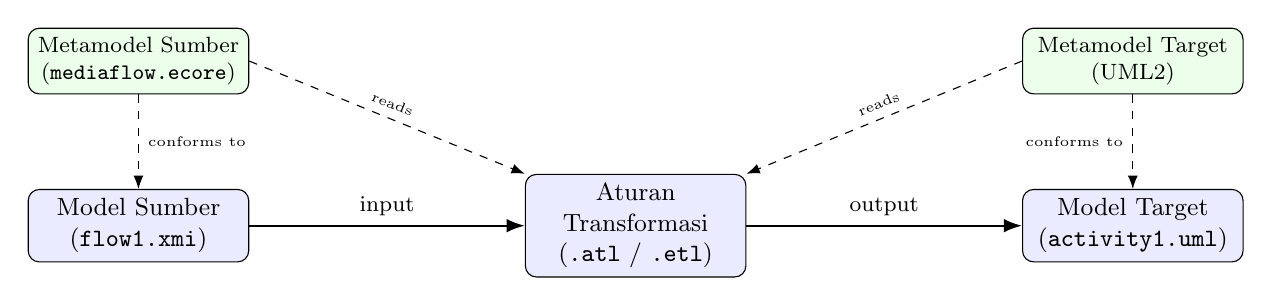
\begin{tikzpicture}[>=Latex, node distance=12mm,
  box/.style={draw,rounded corners,minimum width=2.8cm,minimum height=0.9cm,align=center,fill=blue!8,font=\small},
  mmbox/.style={draw,rounded corners,minimum width=2.8cm,minimum height=0.7cm,align=center,fill=green!8,font=\footnotesize}]
  \node[mmbox] (mm1) {Metamodel Sumber\\(\texttt{mediaflow.ecore})};
  \node[box, below=of mm1] (m1) {Model Sumber\\(\texttt{flow1.xmi})};
  \node[box, right=35mm of m1] (trans) {Aturan\\Transformasi\\(\texttt{.atl} / \texttt{.etl})};
  \node[box, right=35mm of trans] (m2) {Model Target\\(\texttt{activity1.uml})};
  \node[mmbox, above=of m2] (mm2) {Metamodel Target\\(UML2)};
  \draw[->, thick] (m1) -- (trans) node[midway,above,font=\footnotesize]{input};
  \draw[->, thick] (trans) -- (m2) node[midway,above,font=\footnotesize]{output};
  \draw[->, dashed, draw=black] (mm1) -- (m1) node[midway,right,font=\tiny,text=black]{conforms to};
  \draw[->, dashed, draw=black] (mm2) -- (m2) node[midway,left,font=\tiny,text=black]{conforms to};
  \draw[->, dashed, draw=black] (mm1.east) -- (trans.north west) node[midway,above,font=\tiny,sloped,text=black]{reads};
  \draw[->, dashed, draw=black] (mm2.west) -- (trans.north east) node[midway,above,font=\tiny,sloped,text=black]{reads};
\end{tikzpicture}
}

\vspace{6pt}
\small
M2M mengambil model yang berkonformasi ke metamodel sumber dan menghasilkan model yang berkonformasi ke metamodel target, berdasarkan sekumpulan aturan transformasi.
\end{frame}

% ============================================================
\section{Masalah Domain}
\begin{frame}{\hfill}
	\centering
	\Huge{\textbf{Masalah Domain}}
\end{frame}

\begin{frame}{Transformasi: MediaFlow to UML Activity}
\vspace{6pt}
\begin{columns}[T]
\column{0.5\textwidth}
\textbf{Domain Sumber: MediaFlow}
\begin{itemize}
  \item Graf terarah: \texttt{Node}, \texttt{Port}, \texttt{Edge}
  \item Subtipe: \texttt{Resource}, \texttt{Scaler}, \texttt{Transcoder}
  \item Koneksi via Port (\texttt{IN}/\texttt{OUT})
  \item Menyimpan perintah shell di atribut \texttt{command}
\end{itemize}

\column{0.5\textwidth}
\textbf{Domain Target: UML Activity Diagram}
\begin{itemize}
  \item Alur kerja standar UML
  \item \texttt{InitialNode}, \texttt{ActivityFinalNode}
  \item \texttt{OpaqueAction} (aksi dengan body)
  \item \texttt{ControlFlow} (koneksi langsung node-ke-node)
\end{itemize}
\end{columns}

\vspace{8pt}
\small
\textbf{Tantangan utama:} Edge di MediaFlow menghubungkan \texttt{Port} ke \texttt{Port}, tetapi \texttt{ControlFlow} di UML menghubungkan \texttt{Node} ke \texttt{Node} --- transformasi harus menyelesaikan \textit{indirection} ini.
\end{frame}

\begin{frame}{Pemetaan Konseptual}
\vspace{4pt}
\centering
\footnotesize
\begin{tabular}{|>{\raggedright\arraybackslash}p{0.25\textwidth}|>{\raggedright\arraybackslash}p{0.22\textwidth}|>{\raggedright\arraybackslash}p{0.4\textwidth}|}
\hline
\rowcolor{blue!12}
\textbf{MediaFlow} & \textbf{UML} & \textbf{Kondisi} \\
\hline
\texttt{Graph} & \texttt{Model} + \texttt{Activity} & Kontainer root \\
\hline
\texttt{Resource} (entry) & \texttt{InitialNode} & Tidak ada edge masuk \\
\hline
\texttt{Resource} (exit) & \texttt{ActivityFinalNode} & Tidak ada edge keluar \\
\hline
\texttt{Resource} (internal) & \texttt{OpaqueAction} & Ada edge masuk dan keluar; body = URI \\
\hline
\texttt{Scaler} & \texttt{OpaqueAction} & Body = perintah shell \\
\hline
\texttt{Transcoder} & \texttt{OpaqueAction} & Body = perintah shell \\
\hline
\texttt{Edge} & \texttt{ControlFlow} & source/target = owner node dari port \\
\hline
\end{tabular}
\vspace{6pt}

\small
Pemetaan bersifat \textbf{kondisional}: satu tipe sumber (\texttt{Resource}) dipetakan ke 3 tipe target berbeda berdasarkan posisi topologi.
\end{frame}

\begin{frame}{Pemetaan MediaFlow ke UML Activity}
\vspace{10pt}
\begin{figure}
\centering
\scalebox{0.75}{
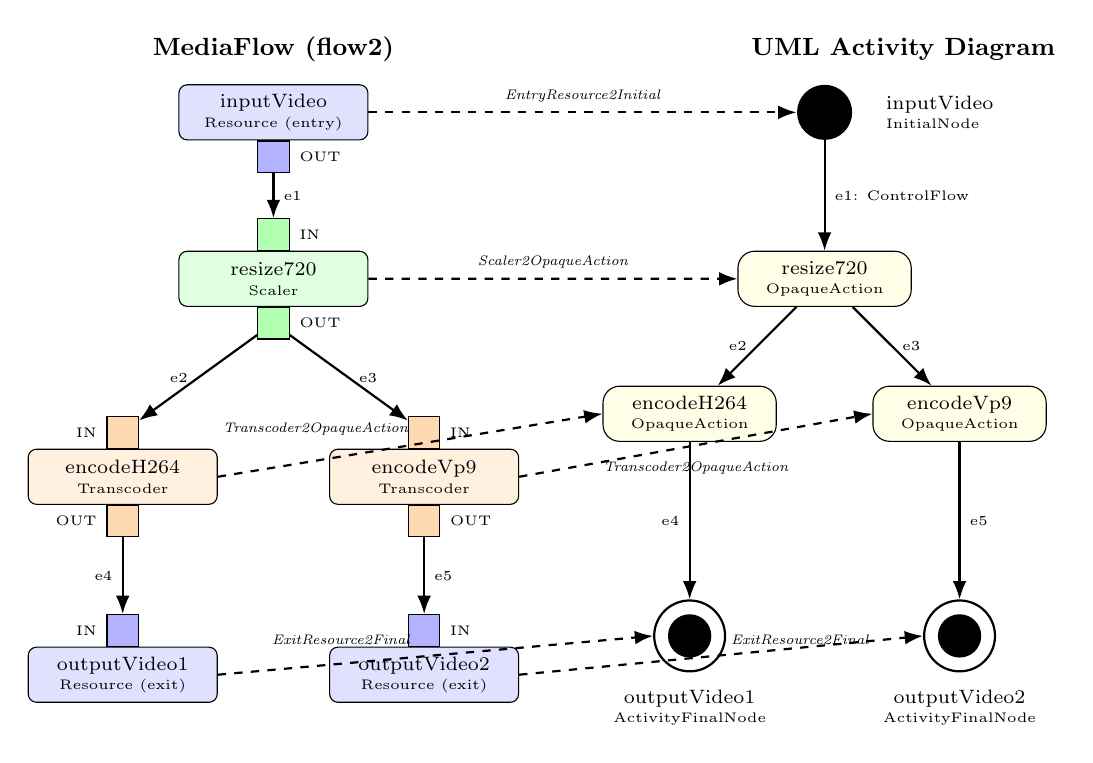
\begin{tikzpicture}[
  >=Latex,
  node distance=8mm,
  mfnode/.style={draw, rounded corners=3pt, minimum width=2.4cm, minimum height=0.7cm, align=center, font=\scriptsize},
  port/.style={draw, fill=white, minimum size=4mm, inner sep=0pt},
  action/.style={draw, rounded corners=6pt, minimum width=2.2cm, minimum height=0.7cm, align=center, font=\scriptsize, fill=yellow!10},
  lbl/.style={font=\tiny\itshape, text=black},
  mapline/.style={->, dashed, draw=black, thick},
  flow/.style={->, thick}
]

  %---------------- LEFT: MEDIAFLOW ----------------%
  \node[font=\small\bfseries] (mftitle) at (0, 0.8) {MediaFlow (flow2)};

  \node[mfnode, fill=blue!12] (res1) at (0, 0) {inputVideo\\[-1pt]{\tiny Resource (entry)}};
  \node[port, fill=blue!30, below=0mm of res1, label={[font=\tiny]right:OUT}] (p-res1-out) {};

  \node[mfnode, fill=green!12, below=14mm of res1] (sc) {resize720\\[-1pt]{\tiny Scaler}};
  \node[port, fill=green!30, above=0mm of sc, label={[font=\tiny]right:IN}] (p-sc-in) {};
  \node[port, fill=green!30, below=0mm of sc, label={[font=\tiny]right:OUT}] (p-sc-out) {};

  \node[mfnode, fill=orange!12, below left=18mm and -5mm of sc] (t1) {encodeH264\\[-1pt]{\tiny Transcoder}};
  \node[port, fill=orange!30, above=0mm of t1, label={[font=\tiny]left:IN}] (p-t1-in) {};
  \node[port, fill=orange!30, below=0mm of t1, label={[font=\tiny]left:OUT}] (p-t1-out) {};

  \node[mfnode, fill=orange!12, below right=18mm and -5mm of sc] (t2) {encodeVp9\\[-1pt]{\tiny Transcoder}};
  \node[port, fill=orange!30, above=0mm of t2, label={[font=\tiny]right:IN}] (p-t2-in) {};
  \node[port, fill=orange!30, below=0mm of t2, label={[font=\tiny]right:OUT}] (p-t2-out) {};

  \node[mfnode, fill=blue!12, below=18mm of t1] (res2) {outputVideo1\\[-1pt]{\tiny Resource (exit)}};
  \node[port, fill=blue!30, above=0mm of res2, label={[font=\tiny]left:IN}] (p-res2-in) {};

  \node[mfnode, fill=blue!12, below=18mm of t2] (res3) {outputVideo2\\[-1pt]{\tiny Resource (exit)}};
  \node[port, fill=blue!30, above=0mm of res3, label={[font=\tiny]right:IN}] (p-res3-in) {};

  \draw[flow] (p-res1-out) -- (p-sc-in) node[midway, right, font=\tiny]{e1};
  \draw[flow] (p-sc-out) -- (p-t1-in) node[midway, left, font=\tiny]{e2};
  \draw[flow] (p-sc-out) -- (p-t2-in) node[midway, right, font=\tiny]{e3};
  \draw[flow] (p-t1-out) -- (p-res2-in) node[midway, left, font=\tiny]{e4};
  \draw[flow] (p-t2-out) -- (p-res3-in) node[midway, right, font=\tiny]{e5};

  %---------------- RIGHT: UML ----------------%
  \node[font=\small\bfseries] (umltitle) at (8, 0.8) {UML Activity Diagram};

  \node[circle, fill=black, minimum size=7mm, inner sep=0pt] (ini) at (7, 0) {};
  \node[font=\scriptsize, right=3mm of ini, align=left] {inputVideo\\[-1pt]{\tiny InitialNode}};

  \node[action, below=14mm of ini] (oa1) {resize720\\[-1pt]{\tiny OpaqueAction}};
  \node[action, below left=10mm and -5mm of oa1] (oa2) {encodeH264\\[-1pt]{\tiny OpaqueAction}};
  \node[action, below right=10mm and -5mm of oa1] (oa3) {encodeVp9\\[-1pt]{\tiny OpaqueAction}};

  \node[circle, draw, thick, minimum size=9mm, inner sep=0pt, below=20mm of oa2] (fin1o) {};
  \node[circle, fill=black, minimum size=5.5mm, inner sep=0pt] at (fin1o.center) (fin1) {};
  \node[font=\scriptsize, below=1mm of fin1o, align=center] {outputVideo1\\[-1pt]{\tiny ActivityFinalNode}};

  \node[circle, draw, thick, minimum size=9mm, inner sep=0pt, below=20mm of oa3] (fin2o) {};
  \node[circle, fill=black, minimum size=5.5mm, inner sep=0pt] at (fin2o.center) (fin2) {};
  \node[font=\scriptsize, below=1mm of fin2o, align=center] {outputVideo2\\[-1pt]{\tiny ActivityFinalNode}};

  \draw[flow] (ini) -- (oa1) node[midway, right, font=\tiny]{e1: ControlFlow};
  \draw[flow] (oa1) -- (oa2) node[midway, left, font=\tiny]{e2};
  \draw[flow] (oa1) -- (oa3) node[midway, right, font=\tiny]{e3};
  \draw[flow] (oa2) -- (fin1o) node[midway, left, font=\tiny]{e4};
  \draw[flow] (oa3) -- (fin2o) node[midway, right, font=\tiny]{e5};

  %---------------- MAPPING LINES ----------------%
  \draw[mapline] (res1.east) -- (ini.west) node[midway, above, lbl]{EntryResource2Initial};
  \draw[mapline] (sc.east) -- (oa1.west) node[midway, above, lbl]{Scaler2OpaqueAction};
  \draw[mapline] (t1.east) -- (oa2.west) node[midway, above, lbl, xshift=-12mm]{Transcoder2OpaqueAction};
  \draw[mapline] (t2.east) -- (oa3.west) node[midway, above, lbl, yshift=-5mm]{Transcoder2OpaqueAction};
  \draw[mapline] (res2.east) -- (fin1o.west) node[midway, above, lbl, xshift=-12mm]{ExitResource2Final};
  \draw[mapline] (res3.east) -- (fin2o.west) node[midway, above, lbl, xshift=10mm]{ExitResource2Final};

\end{tikzpicture}
}

\label{fig:ch11-mapping-visual}
\end{figure}
\end{frame}

\begin{frame}{Masalah Utama}
\vspace{6pt}
\begin{enumerate}
  \item \textbf{Kesenjangan semantik (\textit{semantic gap}).} Koneksi via Port (MediaFlow) vs koneksi langsung node-ke-node (UML). Transformasi harus navigasi dari port ke node pemiliknya.
  \item \textbf{Pemetaan kondisional.} \texttt{Resource} $\rightarrow$ \texttt{InitialNode} / \texttt{ActivityFinalNode} / \texttt{OpaqueAction} berdasarkan analisis topologi.
  \item \textbf{Risiko transformasi manual.} Inkonsistensi meningkat seiring ukuran model. Otomasi memastikan konsistensi deterministik.
  \item \textbf{Portabilitas model.} Output UML bisa dibuka di Eclipse Papyrus --- pemangku kepentingan non-DSL tetap dapat membaca pipeline.
\end{enumerate}
\end{frame}

% ============================================================
\section{Metodologi}
\begin{frame}{\hfill}
	\centering
	\Huge{\textbf{Metodologi Transformasi M2M}}
\end{frame}

\begin{frame}{7 Langkah Metodologi M2M}
\vspace{4pt}
\begin{columns}[T]
\column{0.5\textwidth}
\begin{enumerate}
  \item \textbf{Analisis metamodel} sumber dan target.
  \item \textbf{Perancangan pemetaan} konseptual (tabel mapping).
  \item \textbf{Pemilihan bahasa} transformasi (ATL vs ETL).
  \item \textbf{Definisi helper/operation} untuk navigasi model.
\end{enumerate}

\column{0.5\textwidth}
\begin{enumerate}
  \setcounter{enumi}{4}
  \item \textbf{Penulisan aturan} transformasi.
  \item \textbf{Implementasi runner/launcher} Java.
  \item \textbf{Validasi output} (inspeksi XMI, visualisasi Papyrus, perbandingan ATL vs ETL).
\end{enumerate}
\end{columns}

\vspace{10pt}
\small
\textbf{Dua bahasa digunakan} pada proyek yang sama agar mahasiswa dapat membandingkan paradigma deklaratif (ATL) dan hibrid imperatif-deklaratif (ETL) pada masalah yang identik.
\end{frame}

% ============================================================
\section{Model Input}
\begin{frame}{\hfill}
	\centering
	\Huge{\textbf{Model Input: MediaFlow XMI}}
\end{frame}

\begin{frame}[fragile]{Model Input: \texttt{flow1.xmi} (Linier)}
\vspace{10pt}
\begin{columns}[T]
\column{0.5\textwidth}
\begin{lstlisting}[language=xml, basicstyle=\ttfamily\tiny]
<mediaflow:Graph name="demo">
  <nodes xsi:type="mediaflow:Resource"
      name="inputVideo" uri="file:///home/alfa/videos/input.mp4" external="true">
    <ports name="inputOut" direction="OUT"/>
  </nodes>
  <nodes xsi:type="mediaflow:Scaler" name="resize720" command="ffmpeg -i input.mp4 -vf scale=1280:720 scaled.mp4" replicas="1" width="1280" height="720">
    <ports name="resizeIn"/>
    <ports name="resizeOut" direction="OUT"/>
  </nodes>
  <nodes xsi:type="mediaflow:Resource" name="outputVideo" uri="file:///home/alfa/videos/output.mp4" external="true">
    <ports name="outputIn"/>
  </nodes>
  <edges name="e1" source="//@nodes.0/@ports.0" target="//@nodes.1/@ports.0"/>
  <edges name="e2" source="//@nodes.1/@ports.1" target="//@nodes.2/@ports.0"/>
</mediaflow:Graph>
\end{lstlisting}

\column{0.5\textwidth}
\textbf{Topologi: Linier}\\
\vspace{5pt}
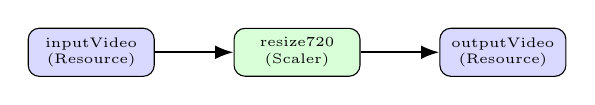
\begin{tikzpicture}[
    >=Latex,
    node distance=10mm,
    box/.style={
        draw,
        rounded corners,
        minimum width=1.6cm,
        minimum height=0.6cm,
        align=center,
        font=\tiny
    }
]
  \node[box,fill=blue!15] (in) {inputVideo\\(Resource)};
  \node[box,fill=green!15,right=of in] (sc) {resize720\\(Scaler)};
  \node[box,fill=blue!15,right=of sc] (out) {outputVideo\\(Resource)};

  \draw[->,thick] (in) -- (sc);
  \draw[->,thick] (sc) -- (out);
\end{tikzpicture}
\vspace{10pt}

\textbf{Poin kunci:}
\begin{itemize}
  \item Edge menghubungkan \texttt{Port} ke \texttt{Port}, bukan node ke node.
  \item \texttt{inputVideo}: hanya port OUT $\rightarrow$ entry.
  \item \texttt{outputVideo}: hanya port IN $\rightarrow$ exit.
\end{itemize}
\end{columns}
\end{frame}

\begin{frame}{Model Input: \texttt{flow2.xmi} (Bercabang)}
\vspace{15pt}
\centering
\scalebox{0.85}{
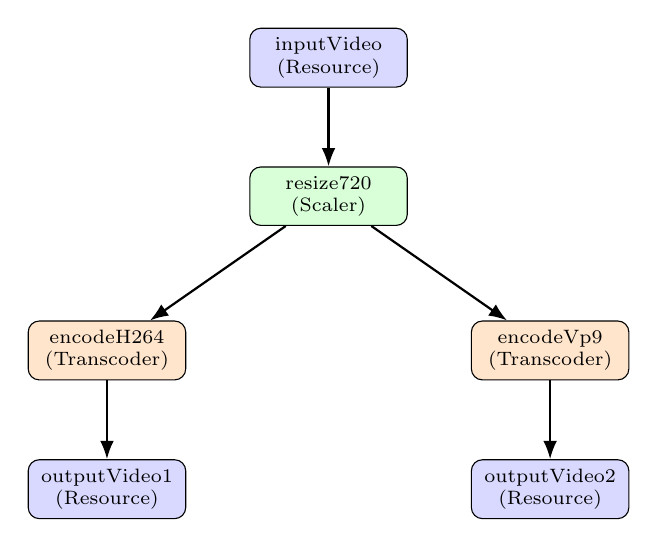
\begin{tikzpicture}[>=Latex, node distance=10mm,
  box/.style={draw,rounded corners,minimum width=2cm,minimum height=0.7cm,align=center,font=\scriptsize}]
  \node[box,fill=blue!15] (in) {inputVideo\\(Resource)};
  \node[box,fill=green!15,below=of in] (sc) {resize720\\(Scaler)};
  \node[box,fill=orange!20,below left=12mm and 8mm of sc] (h264) {encodeH264\\(Transcoder)};
  \node[box,fill=orange!20,below right=12mm and 8mm of sc] (vp9) {encodeVp9\\(Transcoder)};
  \node[box,fill=blue!15,below=of h264] (out1) {outputVideo1\\(Resource)};
  \node[box,fill=blue!15,below=of vp9] (out2) {outputVideo2\\(Resource)};
  \draw[->,thick] (in) -- (sc);
  \draw[->,thick] (sc) -- (h264);
  \draw[->,thick] (sc) -- (vp9);
  \draw[->,thick] (h264) -- (out1);
  \draw[->,thick] (vp9) -- (out2);
\end{tikzpicture}
}

\vspace{6pt}
\small
\texttt{flow2}: 6 node, 5 edge. Satu scaler bercabang ke dua transcoder (H.264 dan VP9).\\
Aturan transformasi harus menangani percabangan dan multiple exit nodes.
\end{frame}

% ============================================================
\section{Implementasi ATL}
\begin{frame}{\hfill}
	\centering
	\Huge{\textbf{Implementasi ATL}}
\end{frame}

\begin{frame}[fragile]{ATL: Header dan Deklarasi Modul}
\vspace{6pt}
\begin{lstlisting}[language=atl]
-- @atlcompiler emftvm
-- @path Mediaflow=platform:/resource/m2m/../mediaflow/metamodels/mediaflow.ecore
-- @path UML=http://www.eclipse.org/uml2/5.0.0/UML

module mediaflow2activity;
create OUT : UML from IN : Mediaflow;
\end{lstlisting}

\vspace{6pt}
\begin{itemize}
  \item \texttt{create OUT : UML from IN : Mediaflow} --- arah transformasi eksplisit.
  \item \texttt{@atlcompiler emftvm} --- dikompilasi ke bytecode EMFTVM.
  \item Paradigma: \textbf{deklaratif, source-driven} --- mesin ATL iterasi semua elemen sumber dan mencocokkan dengan aturan.
\end{itemize}
\end{frame}

\begin{frame}[fragile]{ATL: Helper untuk Navigasi Graf}
\vspace{4pt}
\begin{lstlisting}[language=atl, basicstyle=\ttfamily\tiny]
-- Collect all edges whose target port belongs to this node
helper context Mediaflow!Node def: incomingEdges()
    : Collection(Mediaflow!Edge) =
    Mediaflow!Graph.allInstances()->first().edges
        ->select(e | self.ports->includes(e.target));

-- A node is an entry when nothing flows into it
helper context Mediaflow!Node def: isEntry() : Boolean =
    self.incomingEdges()->isEmpty();

-- A node is an exit when nothing flows out of it
helper context Mediaflow!Node def: isExit() : Boolean =
    self.outgoingEdges()->isEmpty();

-- Resolve the Node that owns the source Port of this edge
helper context Mediaflow!Edge def: sourceNode() : Mediaflow!Node =
    Mediaflow!Graph.allInstances()->first().nodes
        ->any(n | n.ports->includes(self.source));
\end{lstlisting}

\vspace{4pt}
\small
\textbf{6 helper} menyelesaikan indirection port-ke-node: \texttt{incomingEdges}, \texttt{outgoingEdges}, \texttt{isEntry}, \texttt{isExit}, \texttt{sourceNode}, \texttt{targetNode}.
\end{frame}

\begin{frame}[fragile]{ATL: Aturan Graph $\rightarrow$ Model + Activity}
\vspace{4pt}
\begin{lstlisting}[language=atl, basicstyle=\ttfamily\tiny]
rule Graph2Model {
    from g : Mediaflow!Graph
    to
        m : UML!Model (
            name <- g.name + 'Model',
            packagedElement <- Sequence{a}
        ),
        a : UML!Activity (
            name <- g.name + 'Activity',
            ownedNode <-
                Mediaflow!Resource.allInstances()
                    ->union(Mediaflow!Scaler.allInstances())
                    ->union(Mediaflow!Transcoder.allInstances()),
            edge <- Mediaflow!Edge.allInstances()
        )
}
\end{lstlisting}

\vspace{4pt}
\small
\begin{itemize}
  \item Satu elemen sumber (\texttt{Graph}) menghasilkan \textbf{dua} elemen target (\texttt{Model} + \texttt{Activity}).
  \item \texttt{ownedNode} mengumpulkan \textit{semua} instans --- ATL secara otomatis me-resolve ke elemen target yang dihasilkan aturan lain.
\end{itemize}
\end{frame}

\begin{frame}[fragile]{ATL: Aturan Kondisional untuk Resource}
\vspace{7pt}
\begin{columns}[T]
\column{0.58\textwidth}
\begin{lstlisting}[language=atl, basicstyle=\ttfamily\tiny]
-- Entry resource -> InitialNode
rule EntryResource2Initial {
    from r : Mediaflow!Resource(r.isEntry() and not r.isExit())
    to t : UML!InitialNode (
        name <- r.name
    )
}

-- Exit resource -> ActivityFinalNode
rule ExitResource2Final {
    from r : Mediaflow!Resource (r.isExit())
    to t : UML!ActivityFinalNode (
        name <- r.name
    )
}

-- Internal resource -> OpaqueAction
rule InternalResource2Action {
    from r : Mediaflow!Resource(not r.isEntry() and not r.isExit())
    to t : UML!OpaqueAction (
        name <- r.name,
        body <- Sequence{r.uri},
        language <- Sequence{'resource'}
    )
}
\end{lstlisting}

\column{0.44\textwidth}
\vspace{10pt}
\textbf{Pemetaan kondisional}

\vspace{4pt}
Satu tipe sumber (\texttt{Resource}) $\rightarrow$ tiga tipe target:

\vspace{6pt}
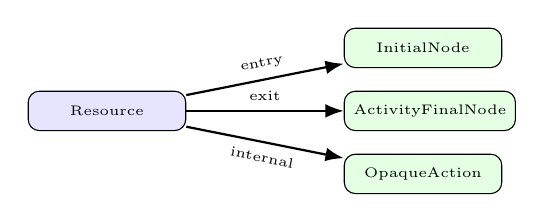
\begin{tikzpicture}[>=Latex, node distance=6mm,
  src/.style={draw,rounded corners,fill=blue!10,minimum width=2cm,minimum height=0.5cm,align=center,font=\tiny},
  tgt/.style={draw,rounded corners,fill=green!10,minimum width=2cm,minimum height=0.5cm,align=center,font=\tiny}]
  \node[src] (r) {Resource};
  \node[tgt, right=20mm of r, yshift=8mm] (ini) {InitialNode};
  \node[tgt, right=20mm of r] (fin) {ActivityFinalNode};
  \node[tgt, right=20mm of r, yshift=-8mm] (opa) {OpaqueAction};
  \draw[->,thick] (r) -- (ini) node[midway,above,font=\tiny,sloped]{entry};
  \draw[->,thick] (r) -- (fin) node[midway,above,font=\tiny]{exit};
  \draw[->,thick] (r) -- (opa) node[midway,below,font=\tiny,sloped]{internal};
\end{tikzpicture}

\vspace{6pt}
\small
Filter pada \texttt{from} menentukan aturan mana yang berlaku berdasarkan predikat topologi (\texttt{isEntry()}, \texttt{isExit()}).
\end{columns}
\end{frame}

\begin{frame}[fragile]{ATL: Aturan Scaler, Transcoder, dan Edge}
\vspace{10pt}
\begin{columns}[T]
    \begin{column}{0.45\textwidth}
\begin{lstlisting}[language=atl, basicstyle=\ttfamily\tiny]
rule Scaler2OpaqueAction {
    from s : Mediaflow!Scaler
    to t : UML!OpaqueAction (
        name <- s.name,
        body <- Sequence{s.command},
        language <- Sequence{'shell'}
    )
}

rule Transcoder2OpaqueAction {
    from t : Mediaflow!Transcoder
    to tt : UML!OpaqueAction (
        name <- t.name,  body <- Sequence{t.command},  language <- Sequence{'shell'}
    )
}

rule Edge2ControlFlow {
    from e : Mediaflow!Edge
    to cf : UML!ControlFlow (
        name <- e.name,
        source <- e.sourceNode(),
        target <- e.targetNode()
    )
}
\end{lstlisting}
    \end{column}

    \begin{column}{0.55\textwidth}

    \textbf{Poin penting}

    \begin{itemize}
        \item \texttt{Scaler} dan \texttt{Transcoder}
        dipetakan menjadi
        \texttt{UML!OpaqueAction}.
        
        \item Properti \texttt{body} berisi
        perintah shell, sedangkan
        \texttt{language} diisi
        \texttt{'shell'}.
        
        \item Aturan \texttt{Edge2ControlFlow}
        membentuk hubungan alur kontrol
        antar node UML.
        
        \item \texttt{sourceNode()} dan
        \texttt{targetNode()} menyelesaikan
        \textit{indirection}, sehingga ATL
        \textbf{otomatis} me-resolve referensi
        ke elemen target yang sesuai
        (\textit{trace-based resolution}).
    \end{itemize}
    \end{column}
\end{columns}
\end{frame}

% ============================================================
\section{Implementasi ETL}
\begin{frame}{\hfill}
	\centering
	\Huge{\textbf{Implementasi ETL}}
\end{frame}

\begin{frame}[fragile]{ETL: Operation untuk Navigasi}
\vspace{4pt}
\begin{lstlisting}[language=etl, basicstyle=\ttfamily\tiny]
operation In!Node incomingEdges() : Collection {
    return In!Graph.all.first().edges.select(edge | self.ports.includes(edge.target));
}

operation In!Node outgoingEdges() : Collection {
    return In!Graph.all.first().edges.select(edge | self.ports.includes(edge.source));
}

operation In!Node isEntry() : Boolean {
    return self.incomingEdges().isEmpty();
}

operation In!Node isExit() : Boolean {
    return self.outgoingEdges().isEmpty();
}

operation In!Edge sourceNode() : In!Node {
    return In!Graph.all.first().nodes.selectOne(node | node.ports.includes(self.source));
}
\end{lstlisting}

\vspace{4pt}
\small
Semantik identik dengan helper ATL, tetapi sintaks lebih mirip bahasa imperatif: \texttt{.select()} tanpa panah, \texttt{.all} tanpa \texttt{allInstances()}.
\end{frame}

\begin{frame}[fragile]{ETL: Aturan Transformasi}
\vspace{4pt}
\begin{columns}[T]
\column{0.45\textwidth}
\begin{lstlisting}[language=etl, basicstyle=\ttfamily\tiny]
rule EntryResource2Initial
    transform source : In!Resource
    to target : Out!InitialNode {
    guard : source.isEntry()
            and not source.isExit()
    target.name = source.name;
}

rule ExitResource2Final
    transform source : In!Resource
    to target : Out!ActivityFinalNode {
    guard : source.isExit()
    target.name = source.name;
}

rule Scaler2OpaqueAction
    transform source : In!Scaler
    to target : Out!OpaqueAction {
    target.name = source.name;
    target.body.add(source.command);
    target.language.add("shell");
}
\end{lstlisting}

\column{0.55\textwidth}
\begin{lstlisting}[language=etl, basicstyle=\ttfamily\tiny]
rule Edge2ControlFlow
    transform source : In!Edge
    to target : Out!ControlFlow {
    target.name = source.name;
    target.source ::= source.sourceNode();
    target.target ::= source.targetNode();
}
\end{lstlisting}

\textbf{Perbedaan dari ATL}

\vspace{4pt}
\begin{enumerate}
  \item \textbf{Assignment imperatif}:\\
  \texttt{target.name = source.name}\\
  bukan \texttt{name <- r.name}

  \vspace{4pt}
  \item \textbf{Operator \texttt{::=}}:\\
  \textit{equivalent binding} --- otomatis resolve ke elemen target yang setara.

  \vspace{4pt}
  \item \textbf{Guard} sebagai pengganti filter \texttt{from}.
\end{enumerate}
\end{columns}
\end{frame}

\begin{frame}[fragile]{ETL: Blok Post --- Pembungkusan ke Activity}
\begin{columns}[T]
    \begin{column}{0.5\textwidth}
\begin{lstlisting}[language=etl, basicstyle=\ttfamily\tiny]
post BuildActivityModel {
    var graph = In!Graph.all.first();
    var rootModel = new Out!Model;
    var activity = new Out!Activity;

    rootModel.name = graph.name + "Model";
    activity.name = graph.name + "Activity";
    rootModel.packagedElement.add(activity);

    for (node in In!Resource.all.equivalent()) {
        activity.ownedNode.add(node);
    }
    for (node in In!Scaler.all.equivalent()) {
        activity.ownedNode.add(node);
    }
    for (node in In!Transcoder.all.equivalent()) {
        activity.ownedNode.add(node);
    }
    for (edge in In!Edge.all.equivalent()) {
        activity.edge.add(edge);
    }
}
\end{lstlisting}
    \end{column}

    \begin{column}{0.5\textwidth}
    \small
    \textbf{Perbedaan arsitektural terbesar}

    \begin{itemize}
        \item ATL membangun kontainer
        (\texttt{Model} dan \texttt{Activity})
        secara deklaratif di aturan
        \texttt{Graph2Model}.
        
        \item ETL melakukannya secara
        \textbf{imperatif} di blok
        \texttt{post}, yaitu dieksekusi
        \textit{setelah} semua aturan selesai.
        
        \item Elemen hasil transformasi diambil
        kembali dengan \texttt{.equivalent()},
        lalu dibungkus ke dalam
        \texttt{Activity}.
    \end{itemize}
    \end{column}
\end{columns}
\end{frame}

% ============================================================
\section{Java Runner}
\begin{frame}{\hfill}
	\centering
	\Huge{\textbf{Java Runner}}
\end{frame}

\begin{frame}{Arsitektur Proyek M2M}
\vspace{4pt}
\centering
\footnotesize
\begin{tabular}{|l|l|}
\hline
\rowcolor{blue!12}
\textbf{Direktori/File} & \textbf{Fungsi} \\
\hline
\texttt{src/m2m/MediaflowToActivityATLRunner.java} & Runner ATL (EMFTVM) \\
\hline
\texttt{src/m2m/MediaflowToActivityETLRunner.java} & Runner ETL (Epsilon) \\
\hline
\texttt{transformer/mediaflow2activity.atl} & Aturan transformasi ATL \\
\hline
\texttt{transformer/mediaflow2activity.emftvm} & Bytecode ATL terkompilasi \\
\hline
\texttt{transformer/mediaflow2activity.etl} & Aturan transformasi ETL \\
\hline
\texttt{input/flow1.xmi}, \texttt{flow2.xmi} & Model input XMI \\
\hline
\texttt{output/activity*atl.uml} & Output ATL \\
\hline
\texttt{output/activity*etl.uml} & Output ETL \\
\hline
\end{tabular}
\end{frame}

\begin{frame}[fragile]{Runner ATL: 5 Tahap Utama}
\vspace{4pt}
\begin{columns}[T]
\column{0.55\textwidth}
\begin{lstlisting}[language=java, basicstyle=\ttfamily\tiny]
// 1. Initialise EMF packages
EcorePackage.eINSTANCE.eClass();
UMLPackage.eINSTANCE.eClass();
EmftvmPackage.eINSTANCE.eClass();

// 2. Register metamodels
Metamodel mediaflowMM = ...;
env.registerMetaModel("Mediaflow", mediaflowMM);
Metamodel umlMM = ...;
env.registerMetaModel("UML", umlMM);

// 3. Load input model
Model inModel = ...;
env.registerInputModel("IN", inModel);

// 4. Execute transformation
env.loadModule(mr, "mediaflow2activity");
env.run(td);

// 5. Save output
outModel.getResource().save(...);
\end{lstlisting}

\column{0.45\textwidth}
\vspace{10pt}
\textbf{Runner ATL lebih kompleks:}
\begin{enumerate}
  \item Registrasi metamodel manual.
  \item Resource factory untuk \texttt{.ecore}, \texttt{.xmi}, \texttt{.emftvm}.
  \item \texttt{ExecEnv} sebagai mesin transformasi.
  \item Bytecode \texttt{.emftvm} \textbf{wajib} ada (hasil kompilasi \texttt{.atl}).
\end{enumerate}
\end{columns}
\end{frame}

\begin{frame}[fragile]{Runner ETL: Lebih Ringkas}
\vspace{6pt}
\begin{columns}[T]
\column{0.5\textwidth}
\begin{lstlisting}[language=java, basicstyle=\ttfamily\tiny]
// Input model (read-only)
EmfModel inputModel = new EmfModel();
inputModel.setName("In");
inputModel.setMetamodelFile(metamodelPath);
inputModel.setModelFile(inputPath);
inputModel.setReadOnLoad(true);
inputModel.setStoredOnDisposal(false);
inputModel.load();

// Output model (write-only)
EmfModel outputModel = new EmfModel();
outputModel.setName("Out");
outputModel.setMetamodelUri(UMLPackage.eNS_URI);
outputModel.setModelFile(outputPath);
outputModel.setReadOnLoad(false);
outputModel.setStoredOnDisposal(true);
outputModel.load();

// Parse and execute
EtlModule module = new EtlModule();
module.parse(new File(transformationPath));
module.getContext().getModelRepository()
    .addModel(inputModel);
module.getContext().getModelRepository()
    .addModel(outputModel);
module.execute();
outputModel.store();
\end{lstlisting}

\column{0.5\textwidth}
\vspace{10pt}
\textbf{Runner ETL lebih ringkas:}
\begin{enumerate}
  \item API \texttt{EmfModel} tingkat tinggi.
  \item Tidak perlu registrasi manual metamodel.
  \item \texttt{EtlModule.parse()} langsung membaca \texttt{.etl} (\textit{interpreted}, tanpa kompilasi).
  \item Try-finally memastikan cleanup resource.
\end{enumerate}
\end{columns}
\end{frame}

% ============================================================
\section{Output dan Evaluasi}
\begin{frame}{\hfill}
	\centering
	\Huge{\textbf{Output dan Evaluasi}}
\end{frame}

\begin{frame}[fragile]{Output: flow1 $\rightarrow$ UML Activity Diagram}
\vspace{4pt}
\begin{columns}[T]
\column{0.55\textwidth}
\begin{lstlisting}[language=xml, basicstyle=\ttfamily\tiny]
<uml:Model name="demoModel">
  <packagedElement xmi:type="uml:Activity"
      name="demoActivity">
    <edge xmi:type="uml:ControlFlow" name="e1"
        target="_opaqueAction"
        source="_initialNode"/>
    <edge xmi:type="uml:ControlFlow" name="e2"
        target="_finalNode"
        source="_opaqueAction"/>
    <node xmi:type="uml:InitialNode"
        name="inputVideo"/>
    <node xmi:type="uml:ActivityFinalNode"
        name="outputVideo"/>
    <node xmi:type="uml:OpaqueAction"
        name="resize720">
      <language>shell</language>
      <body>ffmpeg -i input.mp4 -vf
        scale=1280:720 scaled.mp4</body>
    </node>
  </packagedElement>
</uml:Model>
\end{lstlisting}

\column{0.45\textwidth}
\vspace{10pt}
\textbf{Verifikasi:}
\begin{itemize}
  \item 3 node input $\rightarrow$ 3 ActivityNode
  \item 2 edge input $\rightarrow$ 2 ControlFlow
  \item \texttt{inputVideo} $\rightarrow$ \texttt{InitialNode} {\color{green!60!black}\checkmark}
  \item \texttt{resize720} $\rightarrow$ \texttt{OpaqueAction} {\color{green!60!black}\checkmark}
  \item \texttt{outputVideo} $\rightarrow$ \texttt{ActivityFinalNode} {\color{green!60!black}\checkmark}
  \item Perintah shell dipertahankan di \texttt{body} {\color{green!60!black}\checkmark}
\end{itemize}
\end{columns}
\end{frame}

\begin{frame}{Output: \texttt{flow2} $\rightarrow$ UML Activity Diagram}
\vspace{2pt}
\begin{figure}
\vspace{20pt}
\centering
\scalebox{0.76}{
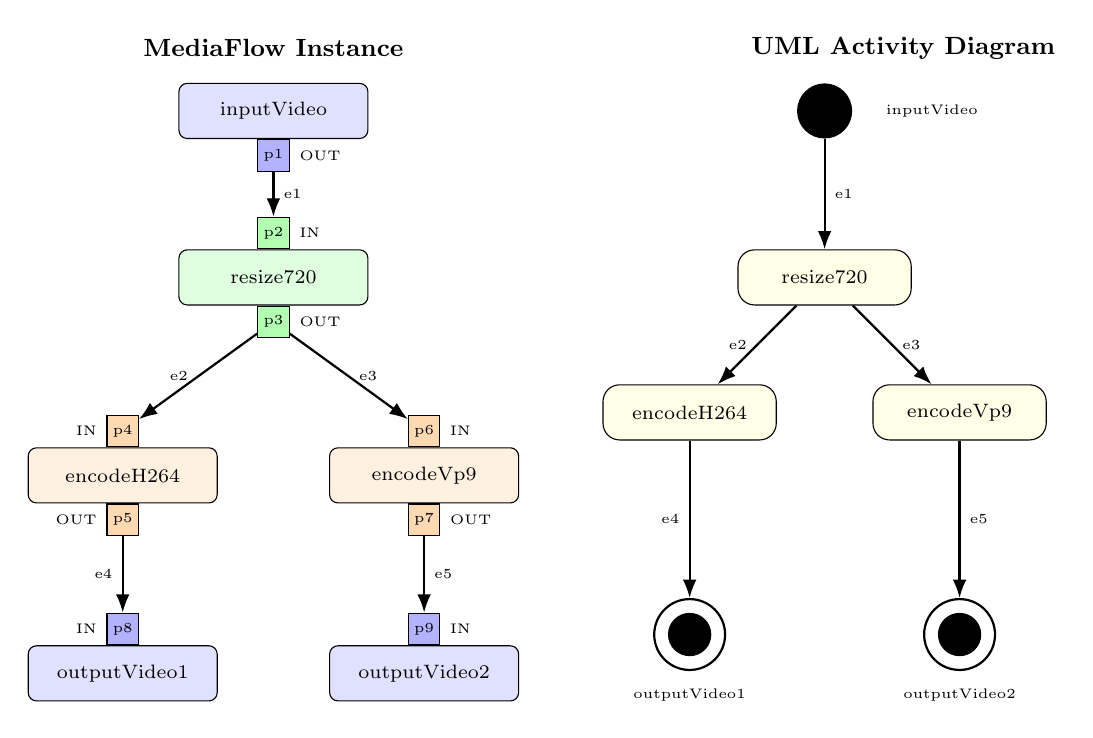
\begin{tikzpicture}[>=Latex, node distance=10mm,
  mfnode/.style={draw, rounded corners=3pt, minimum width=2.4cm, minimum height=0.7cm, align=center, font=\scriptsize},
  port/.style={draw, fill=white, minimum size=4mm, inner sep=0pt, font=\tiny},
  action/.style={draw, rounded corners=6pt, minimum width=2.2cm, minimum height=0.7cm, align=center, font=\scriptsize, fill=yellow!10},
  flow/.style={->, thick}]

  \node[font=\small\bfseries] (mftitle) at (0, 0.8) {MediaFlow Instance};

  \node[mfnode, fill=blue!12] (mf-in) at (0, 0) {inputVideo};
  \node[port, fill=blue!30, below=0mm of mf-in, label={[font=\tiny]right:OUT}] (p-in-out) {p1};

  \node[mfnode, fill=green!12, below=14mm of mf-in] (mf-sc) {resize720};
  \node[port, fill=green!30, above=0mm of mf-sc, label={[font=\tiny]right:IN}] (p-sc-in) {p2};
  \node[port, fill=green!30, below=0mm of mf-sc, label={[font=\tiny]right:OUT}] (p-sc-out) {p3};

  \node[mfnode, fill=orange!12, below left=18mm and -5mm of mf-sc] (mf-h264) {encodeH264};
  \node[port, fill=orange!30, above=0mm of mf-h264, label={[font=\tiny]left:IN}] (p-h264-in) {p4};
  \node[port, fill=orange!30, below=0mm of mf-h264, label={[font=\tiny]left:OUT}] (p-h264-out) {p5};

  \node[mfnode, fill=orange!12, below right=18mm and -5mm of mf-sc] (mf-vp9) {encodeVp9};
  \node[port, fill=orange!30, above=0mm of mf-vp9, label={[font=\tiny]right:IN}] (p-vp9-in) {p6};
  \node[port, fill=orange!30, below=0mm of mf-vp9, label={[font=\tiny]right:OUT}] (p-vp9-out) {p7};

  \node[mfnode, fill=blue!12, below=18mm of mf-h264] (mf-out1) {outputVideo1};
  \node[port, fill=blue!30, above=0mm of mf-out1, label={[font=\tiny]left:IN}] (p-out1-in) {p8};

  \node[mfnode, fill=blue!12, below=18mm of mf-vp9] (mf-out2) {outputVideo2};
  \node[port, fill=blue!30, above=0mm of mf-out2, label={[font=\tiny]right:IN}] (p-out2-in) {p9};

  \draw[flow] (p-in-out) -- (p-sc-in) node[midway, right, font=\tiny]{e1};
  \draw[flow] (p-sc-out) -- (p-h264-in) node[midway, left, font=\tiny]{e2};
  \draw[flow] (p-sc-out) -- (p-vp9-in) node[midway, right, font=\tiny]{e3};
  \draw[flow] (p-h264-out) -- (p-out1-in) node[midway, left, font=\tiny]{e4};
  \draw[flow] (p-vp9-out) -- (p-out2-in) node[midway, right, font=\tiny]{e5};

  \node[font=\small\bfseries] (umltitle) at (8, 0.8) {UML Activity Diagram};

  \node[circle, fill=black, minimum size=7mm, inner sep=0pt] (start) at (7, 0) {};
  \node[font=\tiny, right=3mm of start] {inputVideo};

  \node[action, below=14mm of start] (resize-uml) {resize720};
  \node[action, below left=10mm and -5mm of resize-uml] (h264-uml) {encodeH264};
  \node[action, below right=10mm and -5mm of resize-uml] (vp9-uml) {encodeVp9};

  \node[circle, draw, thick, minimum size=9mm, inner sep=0pt, below=20mm of h264-uml] (end1o) {};
  \node[circle, fill=black, minimum size=5.5mm, inner sep=0pt] at (end1o.center) (end1) {};
  \node[font=\tiny, below=1mm of end1o] {outputVideo1};

  \node[circle, draw, thick, minimum size=9mm, inner sep=0pt, below=20mm of vp9-uml] (end2o) {};
  \node[circle, fill=black, minimum size=5.5mm, inner sep=0pt] at (end2o.center) (end2) {};
  \node[font=\tiny, below=1mm of end2o] {outputVideo2};

  \draw[flow] (start) -- (resize-uml) node[midway, right, font=\tiny]{e1};
  \draw[flow] (resize-uml) -- (h264-uml) node[midway, left, font=\tiny]{e2};
  \draw[flow] (resize-uml) -- (vp9-uml) node[midway, right, font=\tiny]{e3};
  \draw[flow] (h264-uml) -- (end1o) node[midway, left, font=\tiny]{e4};
  \draw[flow] (vp9-uml) -- (end2o) node[midway, right, font=\tiny]{e5};

\end{tikzpicture}
}
\label{fig:ch11-activity-diagram}
\end{figure}
\end{frame}

\begin{frame}{Hasil Evaluasi}
\vspace{6pt}
\centering
\footnotesize
\begin{tabular}{|>{\raggedright\arraybackslash}p{0.15\textwidth}|c|c|c|c|}
\hline
\rowcolor{blue!12}
\textbf{Model Input} & \textbf{Node In} & \textbf{Edge In} & \textbf{Node Out} & \textbf{Edge Out} \\
\hline
\texttt{flow1.xmi} & 3 & 2 & 3 (1 Initial, 1 Opaque, 1 Final) & 2 ControlFlow \\
\hline
\texttt{flow2.xmi} & 6 & 5 & 6 (1 Initial, 3 Opaque, 2 Final) & 5 ControlFlow \\
\hline
\end{tabular}

\vspace{10pt}
\small
\begin{itemize}
  \item Jumlah node dan edge output \textbf{konsisten} dengan model input.
  \item ATL dan ETL menghasilkan model yang \textbf{ekuivalen secara semantik}: nama, tipe, dan konektivitas identik.
  \item Output UML valid dan dapat dibuka di Eclipse Papyrus.
\end{itemize}
\end{frame}

% ============================================================
\section{Perbandingan ATL vs ETL}
\begin{frame}{\hfill}
	\centering
	\Huge{\textbf{Perbandingan ATL vs ETL}}
\end{frame}

\begin{frame}{Perbandingan Aspek Teknis}
\vspace{4pt}
\centering
\scriptsize
\begin{tabular}{|>{\raggedright\arraybackslash}p{0.16\textwidth}|>{\raggedright\arraybackslash}p{0.37\textwidth}|>{\raggedright\arraybackslash}p{0.37\textwidth}|}
\hline
\rowcolor{blue!12}
\textbf{Aspek} & \textbf{ATL} & \textbf{ETL (Epsilon)} \\
\hline
Paradigma & Deklaratif; \textit{matched rules}. & Hibrid imperatif-deklaratif. \\
\hline
Binding & \texttt{name <- r.name} (deklaratif). & \texttt{target.name = source.name} (imperatif). \\
\hline
Resolusi referensi & Otomatis via trace. & Eksplisit via operator \texttt{::=} / \texttt{.equivalent()}. \\
\hline
Kontainer root & Dalam aturan utama (\texttt{Graph2Model}). & Dalam blok \texttt{post} (imperatif, pasca-transformasi). \\
\hline
Kompilasi & Wajib (\texttt{.atl} $\rightarrow$ \texttt{.emftvm}). & Interpreted langsung dari \texttt{.etl}. \\
\hline
Runner complexity & Lebih kompleks. & Lebih ringkas (API \texttt{EmfModel}). \\
\hline
\end{tabular}
\end{frame}

\begin{frame}{Perbandingan Produktivitas}
\vspace{4pt}
\centering
\scriptsize
\begin{tabular}{|>{\raggedright\arraybackslash}p{0.16\textwidth}|>{\raggedright\arraybackslash}p{0.37\textwidth}|>{\raggedright\arraybackslash}p{0.37\textwidth}|}
\hline
\rowcolor{blue!12}
\textbf{Aspek} & \textbf{ATL} & \textbf{ETL (Epsilon)} \\
\hline
Kurva belajar & Sedang; paradigma \textit{matched rule}. & Rendah--sedang; mirip bahasa imperatif. \\
\hline
Debugging & Sulit; binding deklaratif kurang transparan. & Lebih mudah; kode imperatif ditelusuri sekuensial. \\
\hline
Ekspresivitas & Baik untuk pemetaan simetris. & Lebih fleksibel untuk logika imperatif. \\
\hline
Komposisi & Superimposition (overlay aturan). & Import modul dan pewarisan aturan. \\
\hline
Ekosistem & Eclipse M2M, ATL Project. & Platform Epsilon (EOL, EVL, EGL, dll.). \\
\hline
\end{tabular}
\end{frame}

\begin{frame}{Panduan Pemilihan}
\vspace{6pt}
\begin{columns}[T]
\column{0.33\textwidth}
\textbf{Pilih ATL}
\begin{itemize}
  \item Pemetaan simetris \textit{one-to-one} yang jelas.
  \item Tim familiar dengan paradigma deklaratif.
  \item Integrasi ekosistem Eclipse M2M.
\end{itemize}

\column{0.33\textwidth}
\textbf{Pilih ETL}
\begin{itemize}
  \item Logika imperatif signifikan (kontainer pasca-transformasi).
  \item Integrasi bahasa Epsilon lain (EOL, EVL, EGL).
  \item Kemudahan debugging prioritas.
\end{itemize}

\column{0.33\textwidth}
\textbf{Gunakan Keduanya}
\begin{itemize}
  \item Konteks pembelajaran: implementasi sama dalam dua bahasa.
  \item Pemahaman \textit{trade-off} deklaratif vs imperatif lebih mendalam.
\end{itemize}
\end{columns}
\end{frame}

% ============================================================
\section{Risiko dan Pitfall}
\begin{frame}{\hfill}
	\centering
	\Huge{\textbf{Risiko dan Pitfall}}
\end{frame}

\begin{frame}{Pitfall Umum pada M2M}
\vspace{6pt}
\begin{enumerate}
  \item \textbf{Ketidaksesuaian versi metamodel.} Metamodel berubah tanpa update aturan transformasi $\rightarrow$ elemen baru tidak tertangani.
  \item \textbf{Resolusi referensi gagal.} Helper mengembalikan \texttt{null} $\rightarrow$ \texttt{ControlFlow} tanpa \texttt{source}/\texttt{target}.
  \item \textbf{Konflik aturan ATL.} Dua aturan tanpa filter yang memproses tipe sama $\rightarrow$ runtime error.
  \item \textbf{Kompilasi ATL terlupa.} Mengubah \texttt{.atl} tanpa kompilasi ulang \texttt{.emftvm} $\rightarrow$ runner mengeksekusi versi lama.
  \item \textbf{Urutan blok \texttt{post} ETL.} Jika ada beberapa blok \texttt{post}, urutan eksekusi menjadi penting.
  \item \textbf{Dependensi plugin Eclipse.} Versi ATL, Epsilon, UML2, EMF harus konsisten --- ketidaksesuaian memicu \textit{class loading} error.
\end{enumerate}
\end{frame}

% ============================================================
\section{Ringkasan}
\begin{frame}{\hfill}
	\centering
	\Huge{\textbf{Ringkasan}}
\end{frame}

\begin{frame}{Kesimpulan Sesi}
\vspace{6pt}
\begin{itemize}
  \item Transformasi model-ke-model (M2M) adalah mekanisme sentral dalam MDE yang menjembatani model pada domain berbeda secara otomatis dan deterministik.
  \item Implementasi MediaFlow $\rightarrow$ UML Activity Diagram memerlukan 6 helper/operation untuk menyelesaikan indirection port-ke-node dan 6 aturan transformasi.
  \item ATL (deklaratif) membangun kontainer sebagai bagian dari aturan; ETL (hibrid) menggunakan blok \texttt{post} imperatif --- keduanya menghasilkan output yang ekuivalen secara semantik.
  \item ATL unggul pada konsistensi deklaratif untuk pemetaan simetris; ETL unggul pada fleksibilitas imperatif dan kemudahan debugging.
  \item Pemilihan antara keduanya didasarkan pada kompleksitas pemetaan, kebutuhan debugging, dan ekosistem tooling tim.
\end{itemize}
\end{frame}

\end{document}
